% 图 B.1 磁场中电流元受力：dF = I dr x B
\documentclass[tikz,border=5pt]{standalone}
\usetikzlibrary{arrows.meta}
\usepackage{amsmath}
\usepackage{bm}
\usepackage{fontspec}
\setmainfont{Times New Roman}
\begin{document}
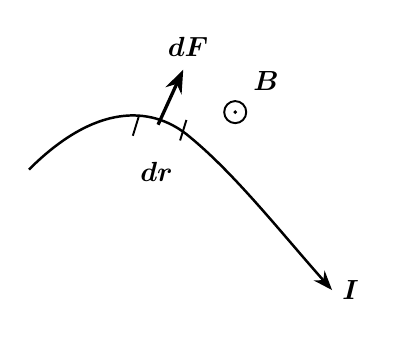
\begin{tikzpicture}[line width=0.8pt,>=Stealth]
% S-shaped wire, current I towards lower right
\draw[line width=0.9pt,->] (0.1,1.55) .. controls (0.95,2.40) and (1.65,2.35)
  .. (2.10,2.00) .. controls (2.70,1.52) and (3.30,0.75) .. (3.95,0.02);
\node[right] at (3.95,0.02) {$\bm{I}$};
% current element dr delimited by two ticks at the crest
\draw[line width=0.7pt] (1.42,1.98) -- (1.50,2.24);
\draw[line width=0.7pt] (2.02,1.92) -- (2.10,2.18);
\node[below] at (1.72,1.78) {$\bm{dr}$};
% force on the element
\draw[line width=1.2pt,->] (1.74,2.12) -- (2.06,2.82);
\node[above] at (2.12,2.86) {$\bm{dF}$};
% B out of the page
\draw[line width=0.7pt] (2.72,2.28) circle (0.14);
\fill (2.72,2.28) circle (0.025);
\node[above right] at (2.82,2.42) {$\bm{B}$};
\end{tikzpicture}
\end{document}
